\author{Mateusz Szulc}
\title{Usuwanie artefaktów kompresji stratnej przy pomocy głębokich sieci neuronowych}
\date{\today}

\documentclass[a4paper, 12pt]{article}


\usepackage[T1]{polski}
\usepackage[utf8]{inputenc}
\usepackage{t1enc}
\usepackage{graphicx}
\usepackage{indentfirst}
\usepackage[belowskip=-10pt,aboveskip=15pt]{caption}
\usepackage[a4paper]{geometry}
\usepackage{listings}

\graphicspath{ {./} }
\setlength\intextsep{5pt}
\setlength{\parindent}{20pt}
\geometry{bottom=2.5cm, top=2.5cm}

\begin{document}
\maketitle
\thispagestyle{empty}
\newpage
\thispagestyle{empty}
Celem dokumentu jest przedstawienie sprawozdania z wykonania projektu w ramach przedmiotu Projekt Indywidualny na semestrze 4 kierunku Informatyka Stosowana Wydziału Elektrycznego PW.
\begin{center}
Projekt realizowany jest pod kierunkiem dr hab. inż. Marcina Iwanowskiego.
\end{center}
\thispagestyle{empty}
\newpage
\tableofcontents
\thispagestyle{empty}

\newpage
\section{Opis problemu}
\indent Projekt ma na celu sprawdzenie możliwości wykorzystania sieci neuronowych typu U-Net do usuwania artefaktów kompresji stratnej JPEG.
Sprawdzone zostały różne architektury sieci, od 1 do 5 poziomów, oraz wpływ rozmiaru segmentu wejściowego na wartość funkcji straty.
Rozwiązanie zostało przystosowane do przetwarzania obrazów o dowolnym, większym niż segment podawany na wejściu sieci, rozmiarze.
\section{Algorytm kompresji JPEG}
Przy niskich wartościach ustawienia jakości, na zapisanych obrazach wyraźny staje się podział zdjęcia na sekcje przez algorytm,
jak i zaburzenia na krawędziach obiektów. Wynikają one z opisanego poniżej sposobu działania algorytmu. \cite{JPEG}
\subsection{Operacje na przestrzeni barw}
W pierwszej kolejności przestrzeń barw RGB konwertowana jest do przestrzeni YCbCr.
Następnie chrominancja jest podpróbkowana, w wyniku czego każdy piksel obrazu wyjściowego stanowi średnią 4 pikseli obrazu wejściowego.
Następuje utrata danych ale jest mało odczuwalna ze względu budowę ludzkiego oka.
\subsection{Dyskretna transformata kosinusowa}
Obraz zostaje podzielony na segmenty 8x8 pikseli, odjęte zostaje 128 od wartości każdego piksela.
Każdy z segmentów zostaje przekształcony w macierz, obrazującą użycie poszczególnych bloków dyskretnej transformaty kosinusowej.
\begin{figure}[h!]
	\begin{center}
	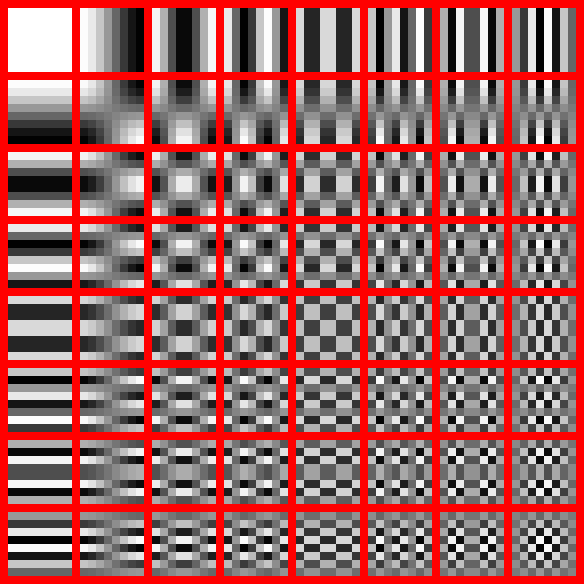
\includegraphics[width=0.4\columnwidth]{DCT.png}
	\caption{Dyskretna Transformata Kosinusowa}
\end{center}
\end{figure}
\\
Sumując wartości pikseli z wybranych bloków, możemy uzyskać dowolną kombinację 8x8 pikseli.
\subsection{Kwantyzacja}
W kolejnym kroku następuje zmniejszenie ilości bitów potrzebnych do reprezentacji wartości pikseli.
Wartości z macierzy są dzielone przez odpowiadające wartości, odwrotnie proporcjonalne do wybranego ustawienia jakości, z tablicy kwantyzacji.
Współczynniki w tablicy kwantyzacji rosną, zmierzając do dolnej, prawej części macierzy.
Odpowiada to zwiększaniu się zagęszczenia informacji w tablicy bloków wykorzystanej w poprzednim kroku.
Taka operacja wykorzystuje problem z rozróżnieniem informacji o dużym zagęszczeniu przez ludzkie oko.
Otrzymane wartości są zaokrąglane do najbliższej liczby całkowitej, następuje utrata danych.
\subsection{Kodowanie}
Otrzymana macierz jest spłaszczana według następującego wzorca:
\begin{figure}[h!]
	\begin{center}
	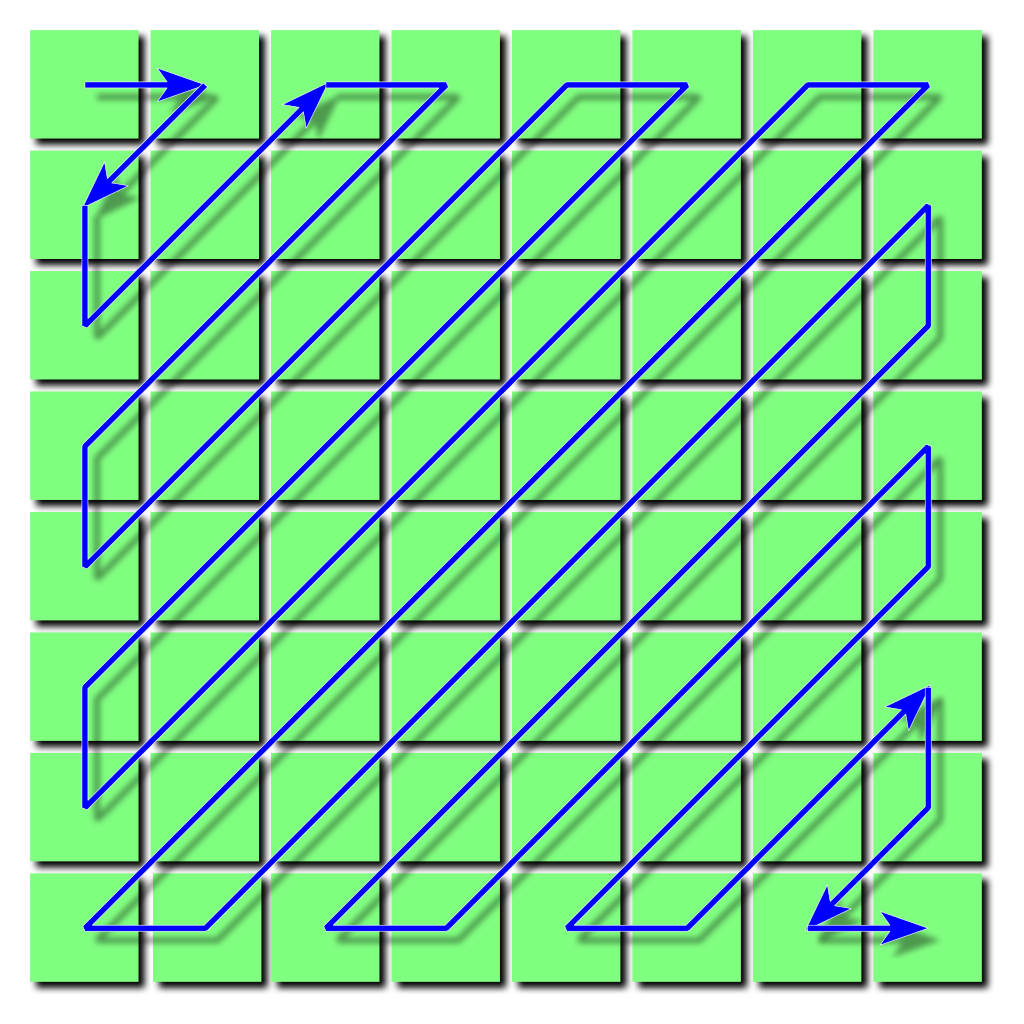
\includegraphics[width=0.5\columnwidth]{pattern.png}
	\caption{Kolejność spłaszczania segmentu}
\end{center}
\end{figure}
\\
Co zwiększa prawdopodobieństwo wystąpienia długich sekwencji zer, możliwych do zapisania w zwięźlejszy sposób.
Na koniec obraz zostaje poddany kompresji kodowaniem Huffmana.
\newpage
\section{Sieci typu U-Net}
U-Net jest architekturą sieci konwolucyjnch, najczęściej stosowaną do segmentacji semantycznej obrazów \cite{ronneberger2015unet}.
Udokumentowane zostały również próby wykorzystania architektury do usuwania zakłóceń z obrazu \cite{antholzer2018deep} .
Wyróżnić można 2 części sieci U-Net.
\begin{figure}[h!]
	\begin{center}
	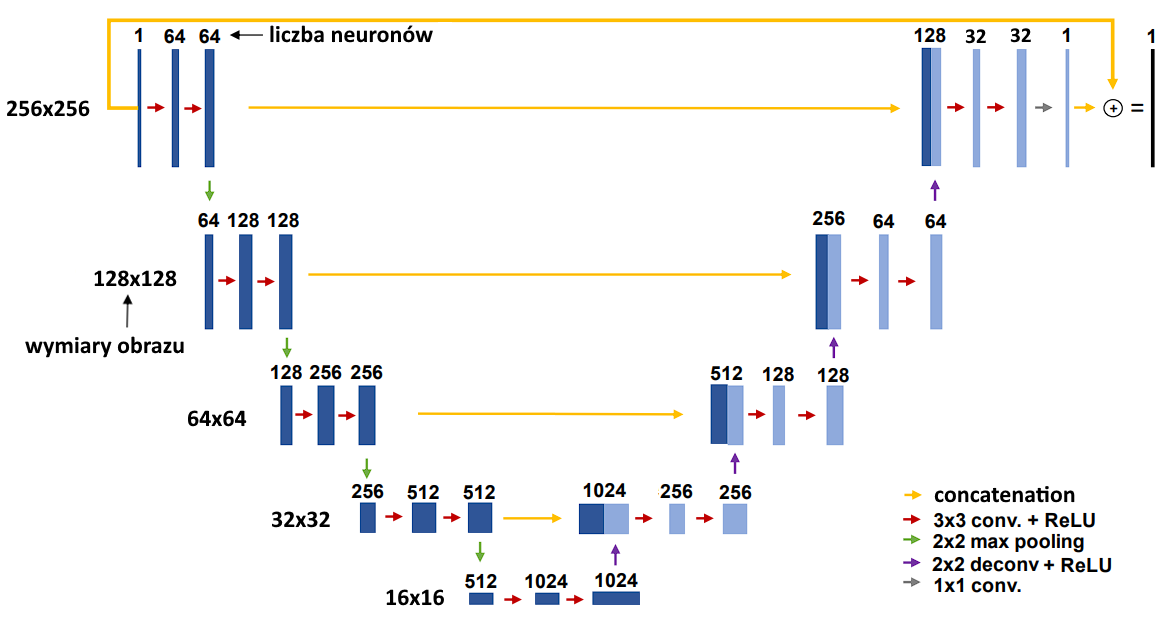
\includegraphics[width=0.9\columnwidth]{unet.png}
	\caption{Zastosowana w projekcie architektura sieci U-Net o 5 poziomach \cite{ronneberger2015unet}}
\end{center}
\end{figure}
\subsection{Enkoder}
Pierwszą częścią modelu jest warstwa wejściowa, w której każdemu pikselowi monochromatycznego segmentu wejściowego odpowiada 1 neuron.
Następne są 2 etapy konwolucji o jądrze 3x3 oraz funkcji aktywacji ReLu, zwiększające liczbę neuronów do 64.
Kolejne są powtarzalne segmenty składające się z redukcji rozdzielczości segmentu i konwolucji z funkcją aktywacji ReLu.
Skutkuje to czterokrotnym zmniejszeniem rozmiaru segmentu oraz podwojeniem liczby neuronów w każdej warstwie.
\lstset{language=Python}
\lstset{frame=lines}
\lstset{caption={Implementacja warstwy enkodera w bibliotece Keras}}
\lstset{label={lst:code_direct}}
\lstset{basicstyle=\footnotesize}
\begin{lstlisting}
pooling = layers.MaxPooling2D(pool_size=2, strides=2)(input)
conv = layers.Conv2D(
    neurons_number, kernel_size=3, padding="same", activation="relu"
)(pooling)
layers.Conv2D(
    neurons_number, kernel_size=3, padding="same", activation="relu"
)(conv)
\end{lstlisting}
\newpage

\subsection{Dekoder}
Każda z powtarzalnych warstw dekodera składa się z 3 elementów.
Pierwsza jest transponowana konwolucja o jądrze 2x2. Następnie powstała sieć jest łączona z odpowiadającą jej warstwą enkodera.
Takie połączenie przeciwdziała problemowi zanikającego gradientu - przywraca cechy wykryte w poprzednich warstwach sieci.
Po niej znajdują się 2 warstwy konwolucji z funkcją aktywacji ReLu.
\lstset{language=Python}
\lstset{frame=lines}
\lstset{caption={Implementacja warstwy dekodera w bibliotece Keras}}
\lstset{label={lst:code_direct}}
\lstset{basicstyle=\footnotesize}
\begin{lstlisting}
tconv = layers.Conv2DTranspose(
    neurons_number, kernel_size=2, strides=(2, 2), activation="relu"
)(input)
concat = layers.Concatenate(axis=3)([tconv, connected_layer])
dconv = layers.Conv2D(
    neurons_number / 2, kernel_size=3, padding="same", activation="relu"
)(concat)
layers.Conv2D(
    neurons_number / 2, kernel_size=3, padding="same", activation="relu"
)(dconv)
\end{lstlisting}

Dekoder zakończony jest spłaszczeniem segmentu do postaci, w której każdy neuron odpowiada 1 pikselowi segmentu wyjściowego.
Warstwa wyjściowa jest sumą segmentu wejściowego i spłaszczonej warstwy.
Przy takim rozwiązaniu, zwanym połączeniami rezydualnymi, sieć tworzy maskę zmian potrzebnych w segmencie wejściowym,
zamiast bezpośrednio przekształcać segment. \cite{he2015deep}

\section{Generacja zbioru danych}
Zbiór danych stanowi 16 kolorowych zdjęć wysokiej rozdzielczości, 1 monochromatyczny wykres służący do kalibracji sprzętu fotograficznego,
oraz 3 wygenerowane obrazy składające się z gradientów kolorów i prostych kształtów.
Zdjęcia zostają podzielone na warstwy RGB i pocięte na kwadratowe segmenty o zadanym rozmiarze.
Wygenerowane zostają wszystkie możliwe kombinacje obróceń i odbić segmentów.
Oryginały segmentów zostają zapisane przy parametrze jakości wynoszącym 100.
Zbiór zostaje podzielony na dane uczące i testowe w proporcji 9:1.
Segmenty zostają zapisane przy ustawieniu jakości równym 25, przy którym artefakty kompresji zaczynają być łatwo zauważalne.
W przypadku podziału na segmenty o rozmiarze 256x256 pikseli otrzymujemy 9500 próbek w zbiorze testowym, oraz 1000 w zbiorze walidacyjnym.
\begin{figure}[h!]
\begin{center}
	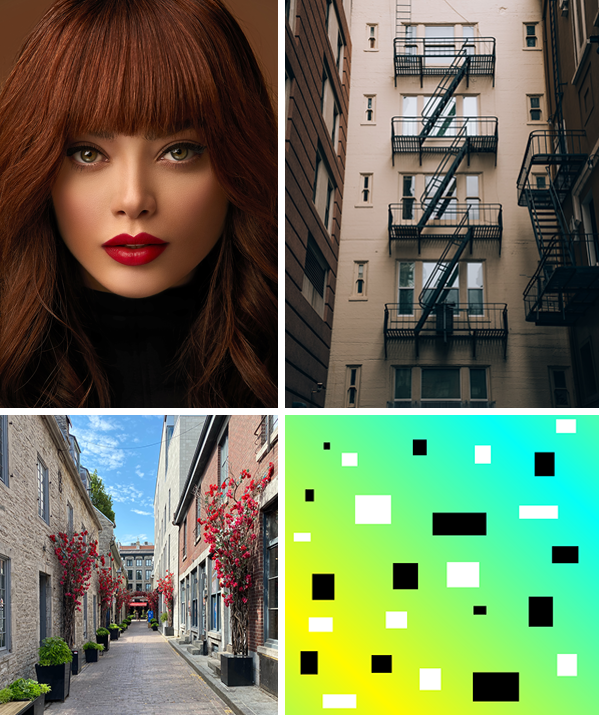
\includegraphics[width=0.85\columnwidth]{dataset.png}
	\caption{Przykładowe obrazy ze zbioru danych}
\end{center}
\end{figure}

\newpage
\section{Model i szkolenie}
Podstawową architekturą w projekcie jest, najczęściej stosowana, sieć o 5 poziomach. \cite{ronneberger2015unet}
Do procesu uczenia utworzone zostają generatory danych testowych i walidacyjnych.
Zawierają one skompresowane oraz oryginalne segmenty, te drugie wykorzystywane w modelu jako maska.
Pogrupowane zostają w paczki po 3.
Podczas jednego kroku uczenia, wykorzystane zostaje, losowo wybrane, 10\% paczek ze zbioru uczącego.
Proces uczenia trwa 100 epok.
Dane uczące i walidacyjne wybierane są na podstawie stałego ziarna, co pozwala na porównanie wyników modeli.
Jako funkcję straty wybrana została wartość bezwzględna błędu, optymalizator to Adam o współczynniku uczenia 0,0001.

\begin{figure}[h!]
\begin{center}
	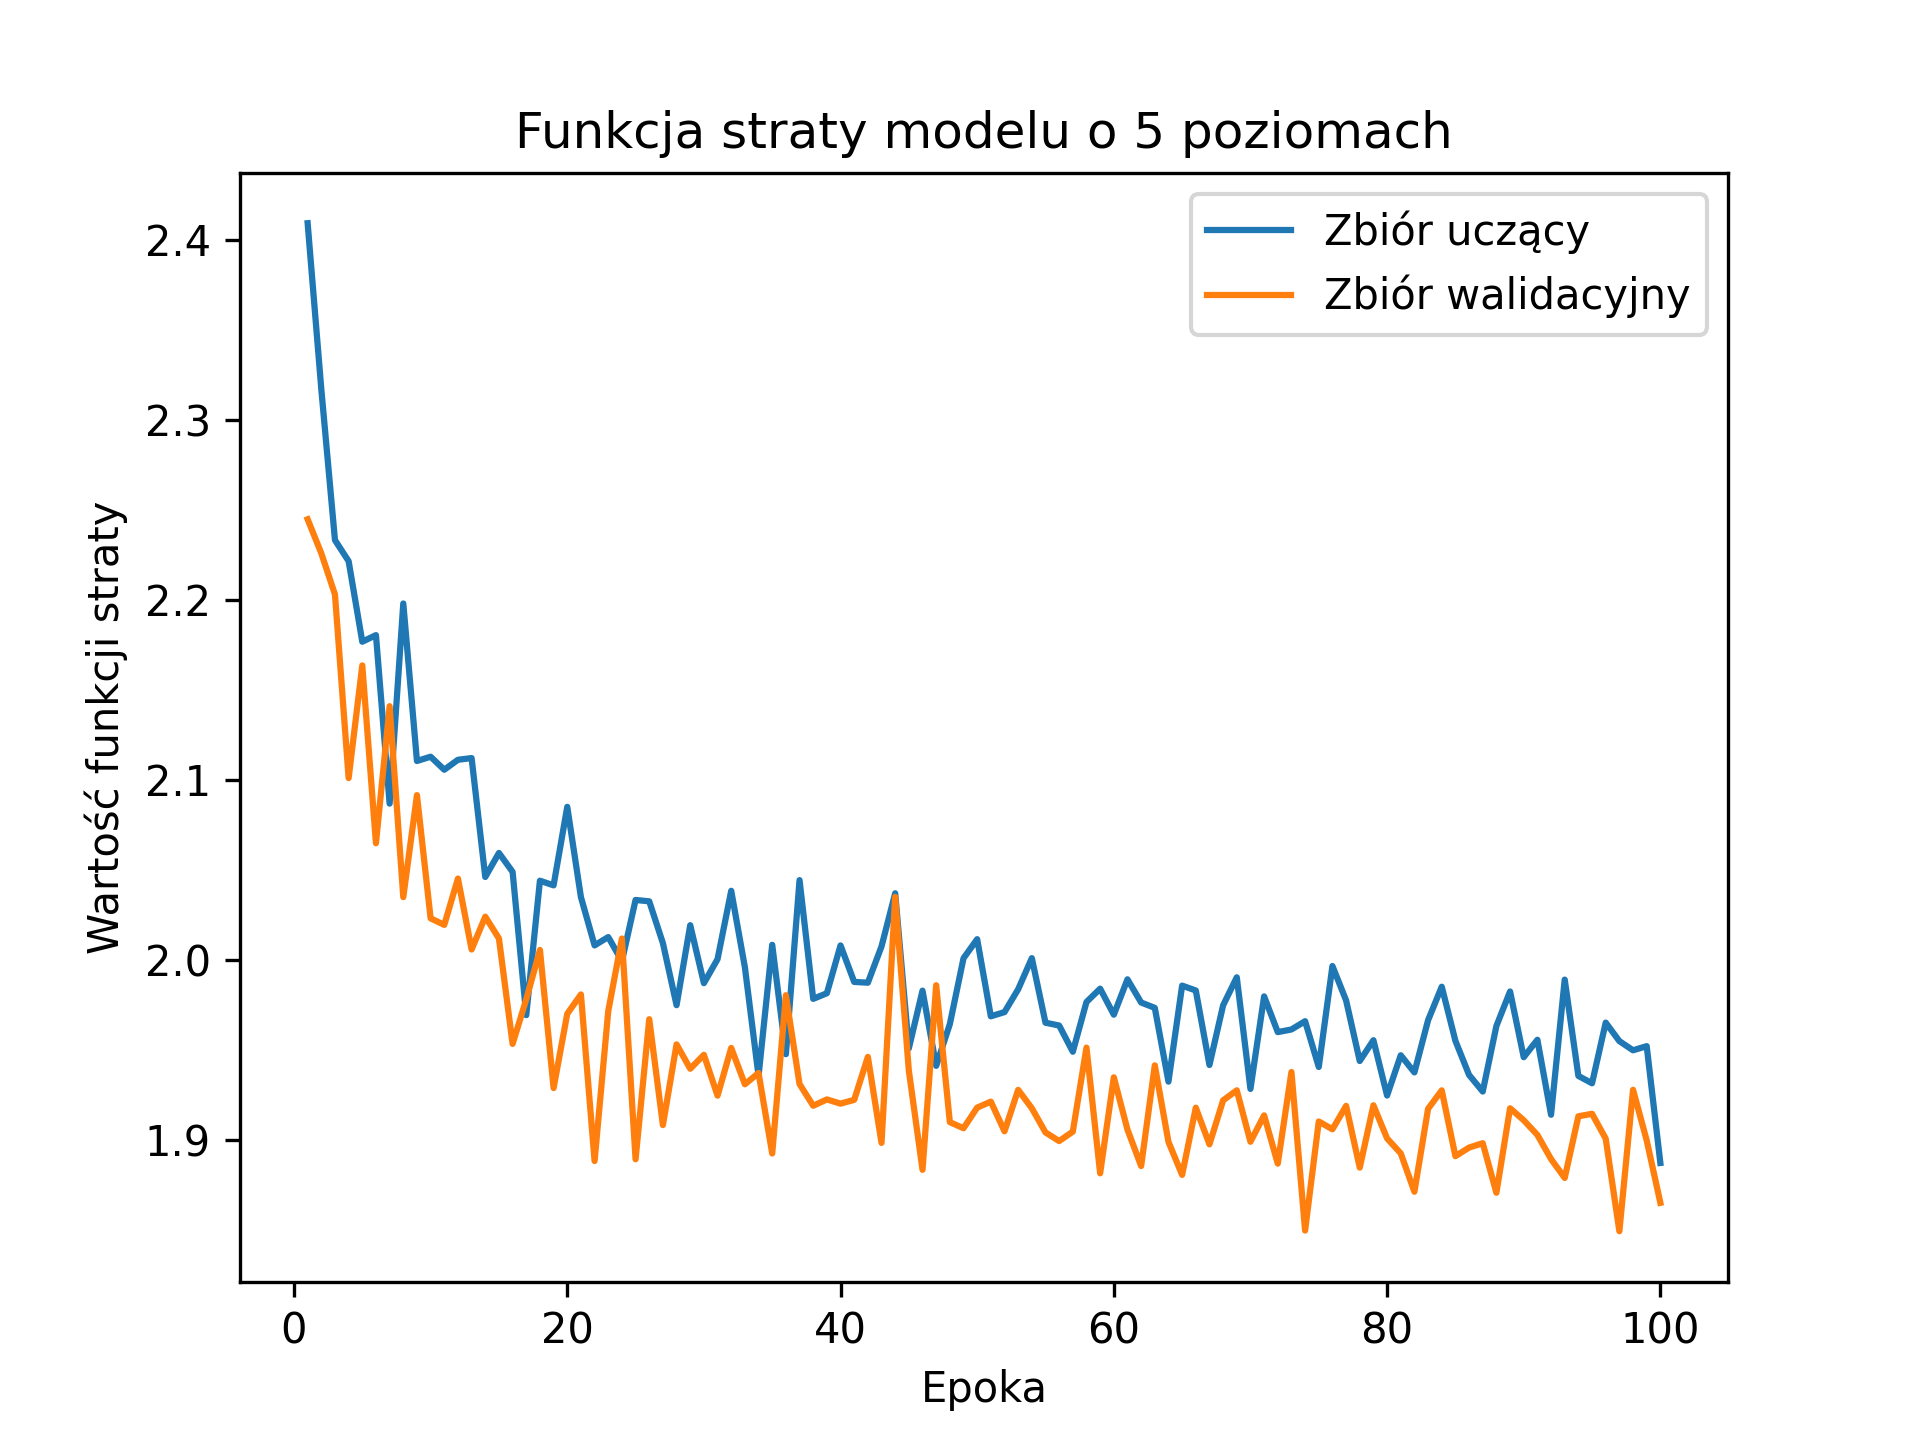
\includegraphics[width=0.7\columnwidth]{loss5.png}
	\caption{Funkcja straty}
\end{center}
\end{figure}

Zauważyć można, że po 20 epoce, tempo zmniejszania wartości funkcji straty znacząco maleje,
a po 60 epoce praktycznie zatrzymuje.
Wartym uwagi jest niższa wartość straty w zbiorze walidacyjnym niż uczącym. Jako że zbiory zostały utworzone z tych samych zdjęć,
prawdopodobnie jest, że to losowy przypadek w wybranym ziarnie generatora danych.
Podczas uczenia dokładność była znikoma i stała. Nie jest ona jednak miarodajną metryką, gdyż oczekuje dokładnych wartości pikseli.
Człowiek nie rozpoznaje małych różnic w wartościach RGB, w związku z czym ważna była jedynie wartość funkcji straty.
\newpage
\section{Wybór optymalnej architektury}
Ważna przy wyborze architektury sieci jest jej złożoność, nadmierna negatywnie wpływa na czas uczenia pomimo znikomej poprawy wartości funkcji błędu.
\subsection{Liczba poziomów sieci}
Przetestowane zostały sieci od 1 do 5 poziomów. Każda została wyszkolona w takich samych warunkach i przy stałym ziarnie generatora danych.
\begin{figure}[h!]
\begin{center}
	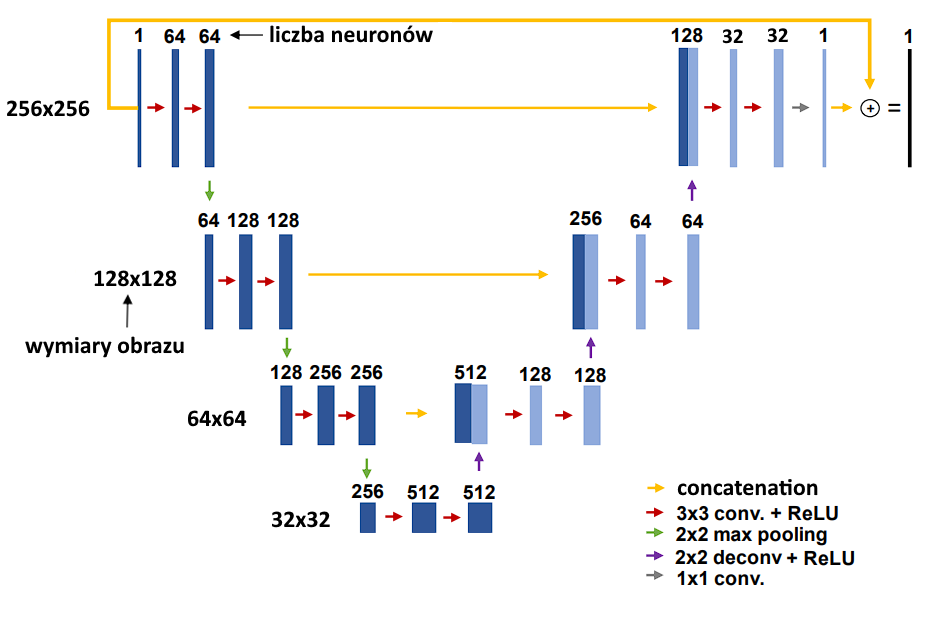
\includegraphics[width=0.9\columnwidth]{unet4.png}
	\caption{Architektura sieci U-Net o 4 poziomach}
\end{center}
\end{figure}
\newpage
\newgeometry{bottom=0.1cm, top=0.1cm}
\begin{figure}[h!]
\begin{center}
	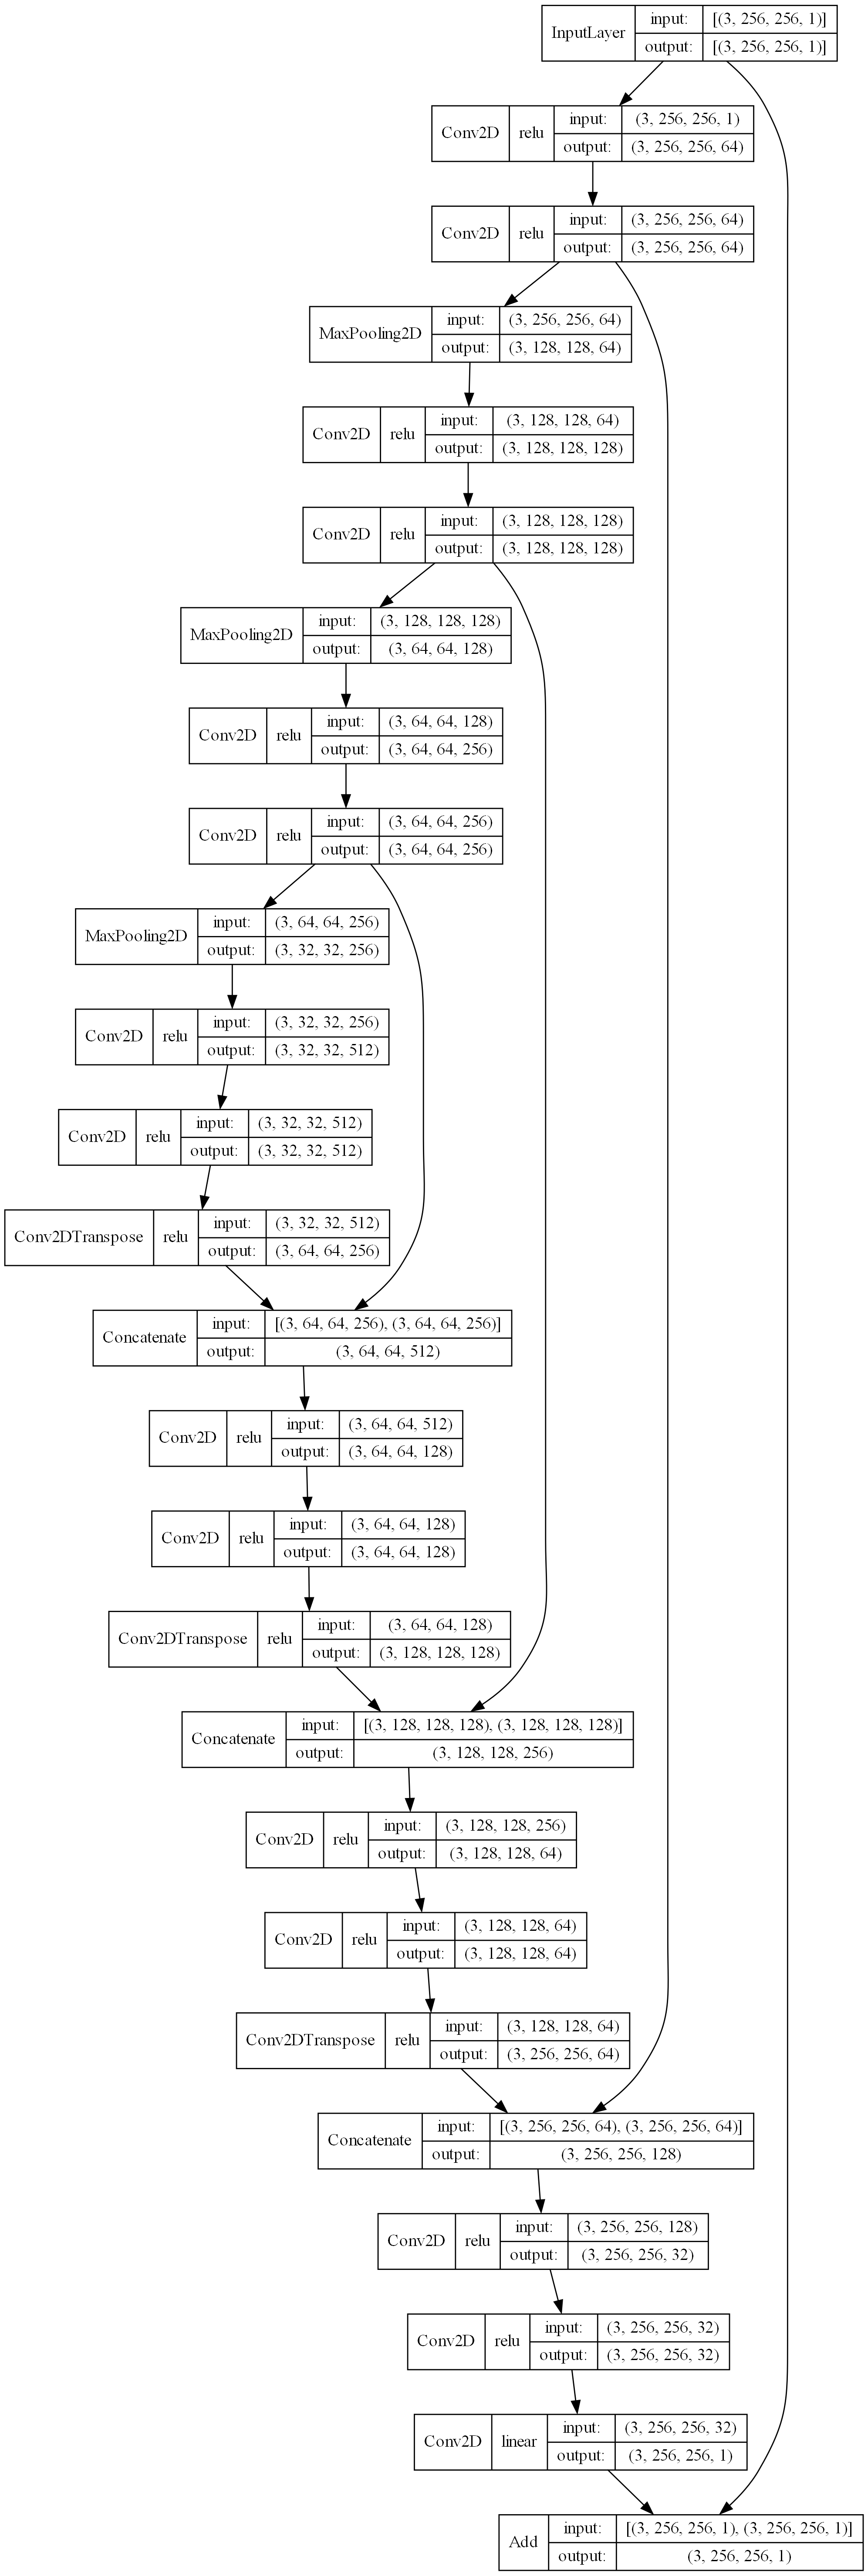
\includegraphics[height=0.95\paperheight]{model_plot.png}
	\caption{Graf obrazujący sieć U-Net o 4 poziomach zaimplementowaną w Keras}
\end{center}
\end{figure}
\thispagestyle{empty}
\newpage
\restoregeometry
\begin{figure}[h!]
\begin{center}
	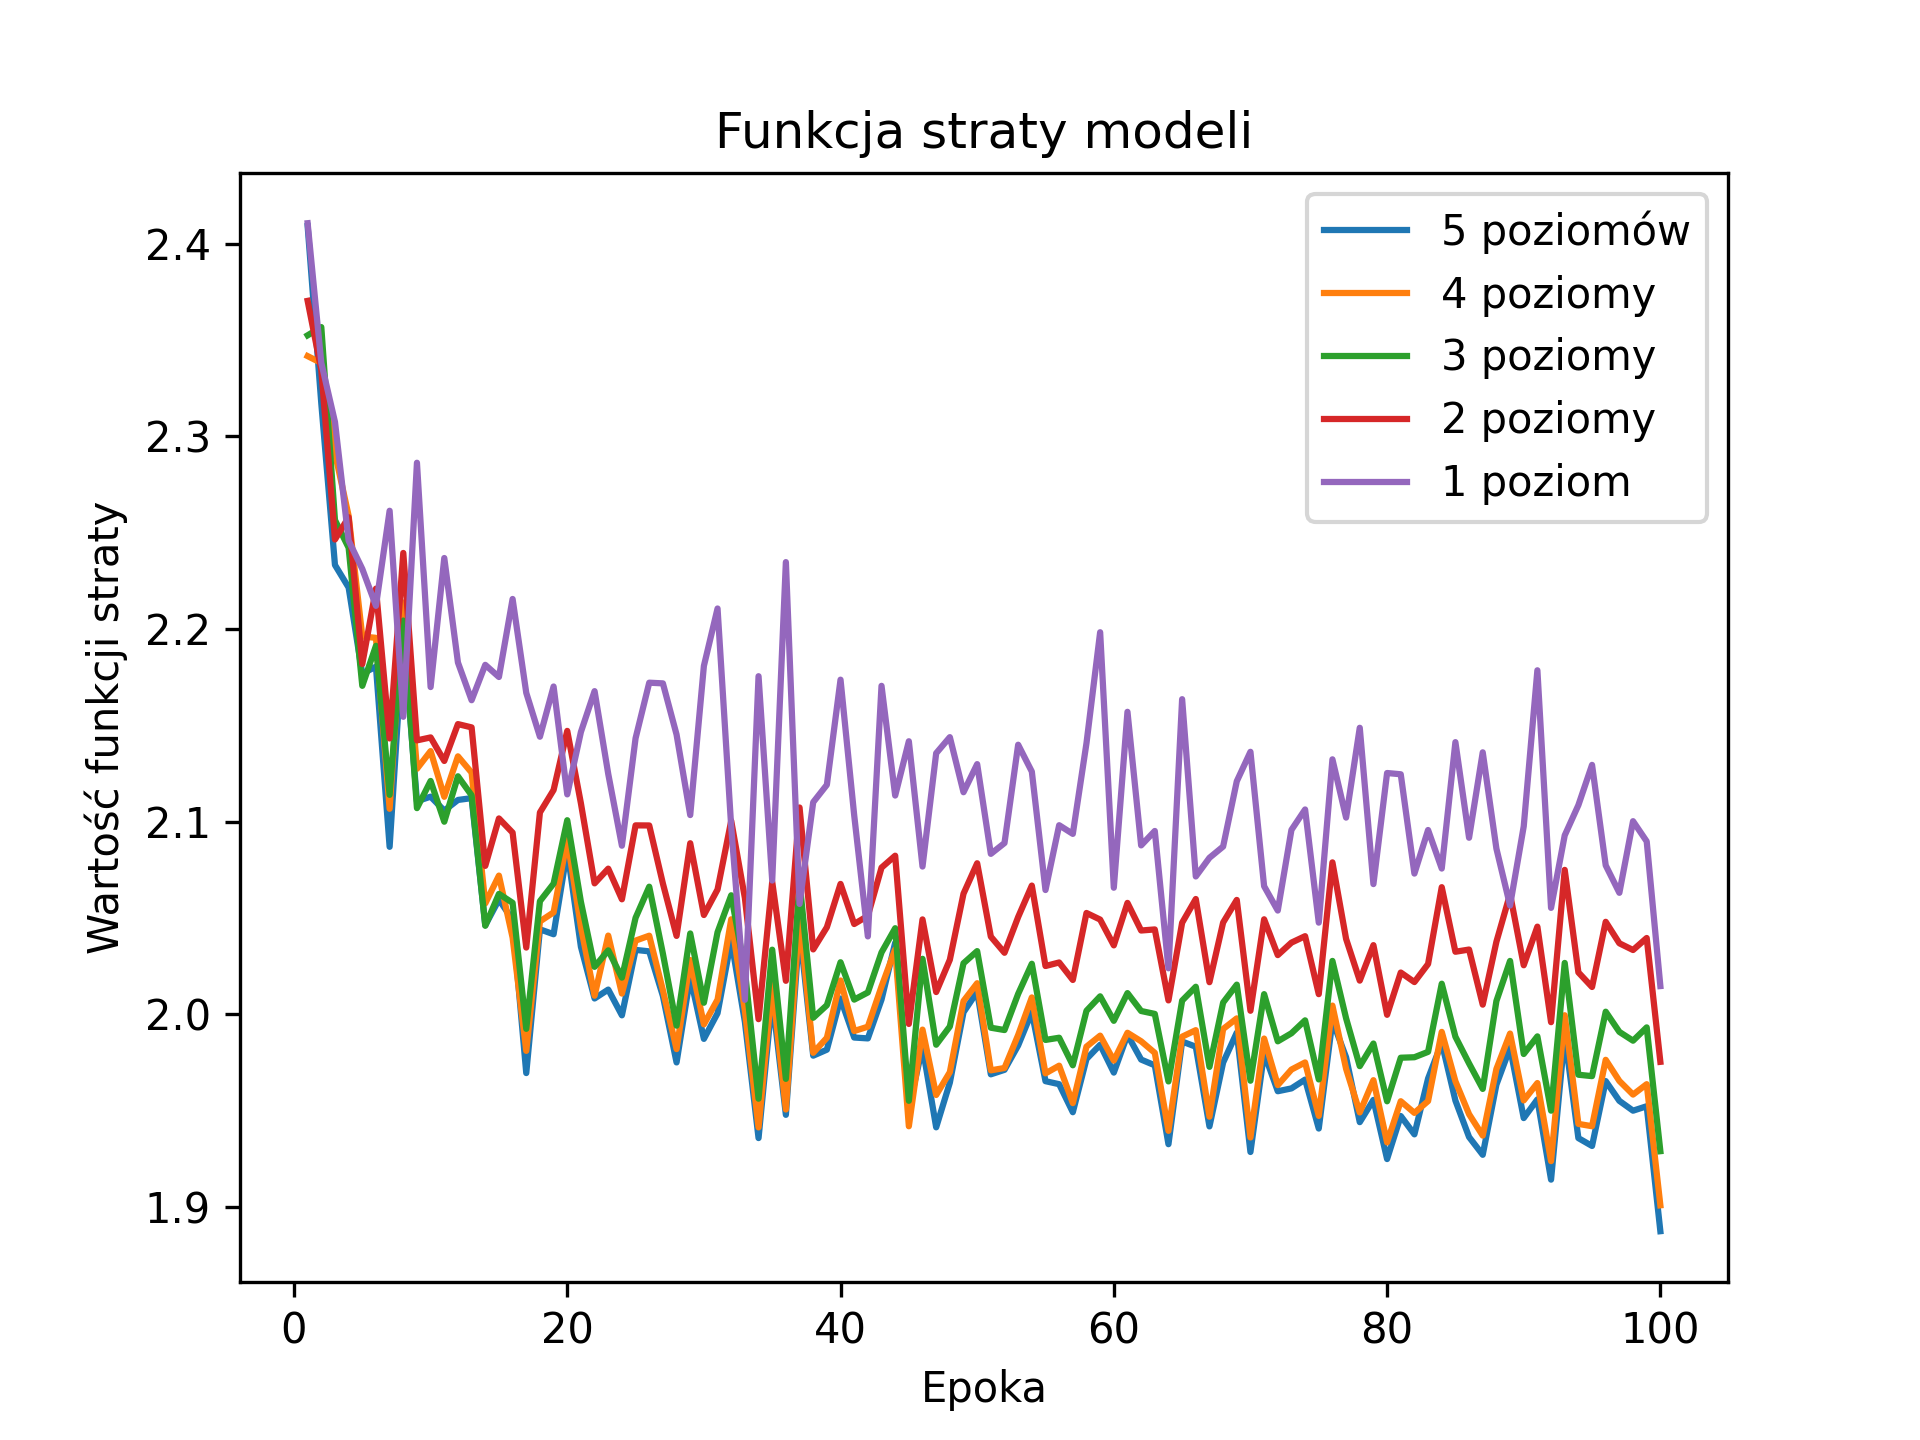
\includegraphics[width=0.7\columnwidth]{layers.png}
	\caption{Funkcja straty przy różnej liczbie poziomów sieci}
\end{center}
\end{figure}
Zauważyć można zbliżone wyniki sieci o 3, 4 i 5 poziomach.
Dla 1 i 2 poziomów wystąpiło znaczące pogorszenie wyników. Zmiana wartości funkcji straty spowolniła przy podobnej liczbie epok.
Wynika z tego, że do problemu wystarczy zastosowania sieci o 3 lub 4 poziomach, co przyśpieszy proces uczenia.
\subsection{Rozmiar segmentu wejściowego}
Przetestowany został również wpływ rozmiaru segmentu wejściowego na wartość funkcji straty przy 4 poziomach sieci.
\begin{figure}[h!]
\begin{center}
	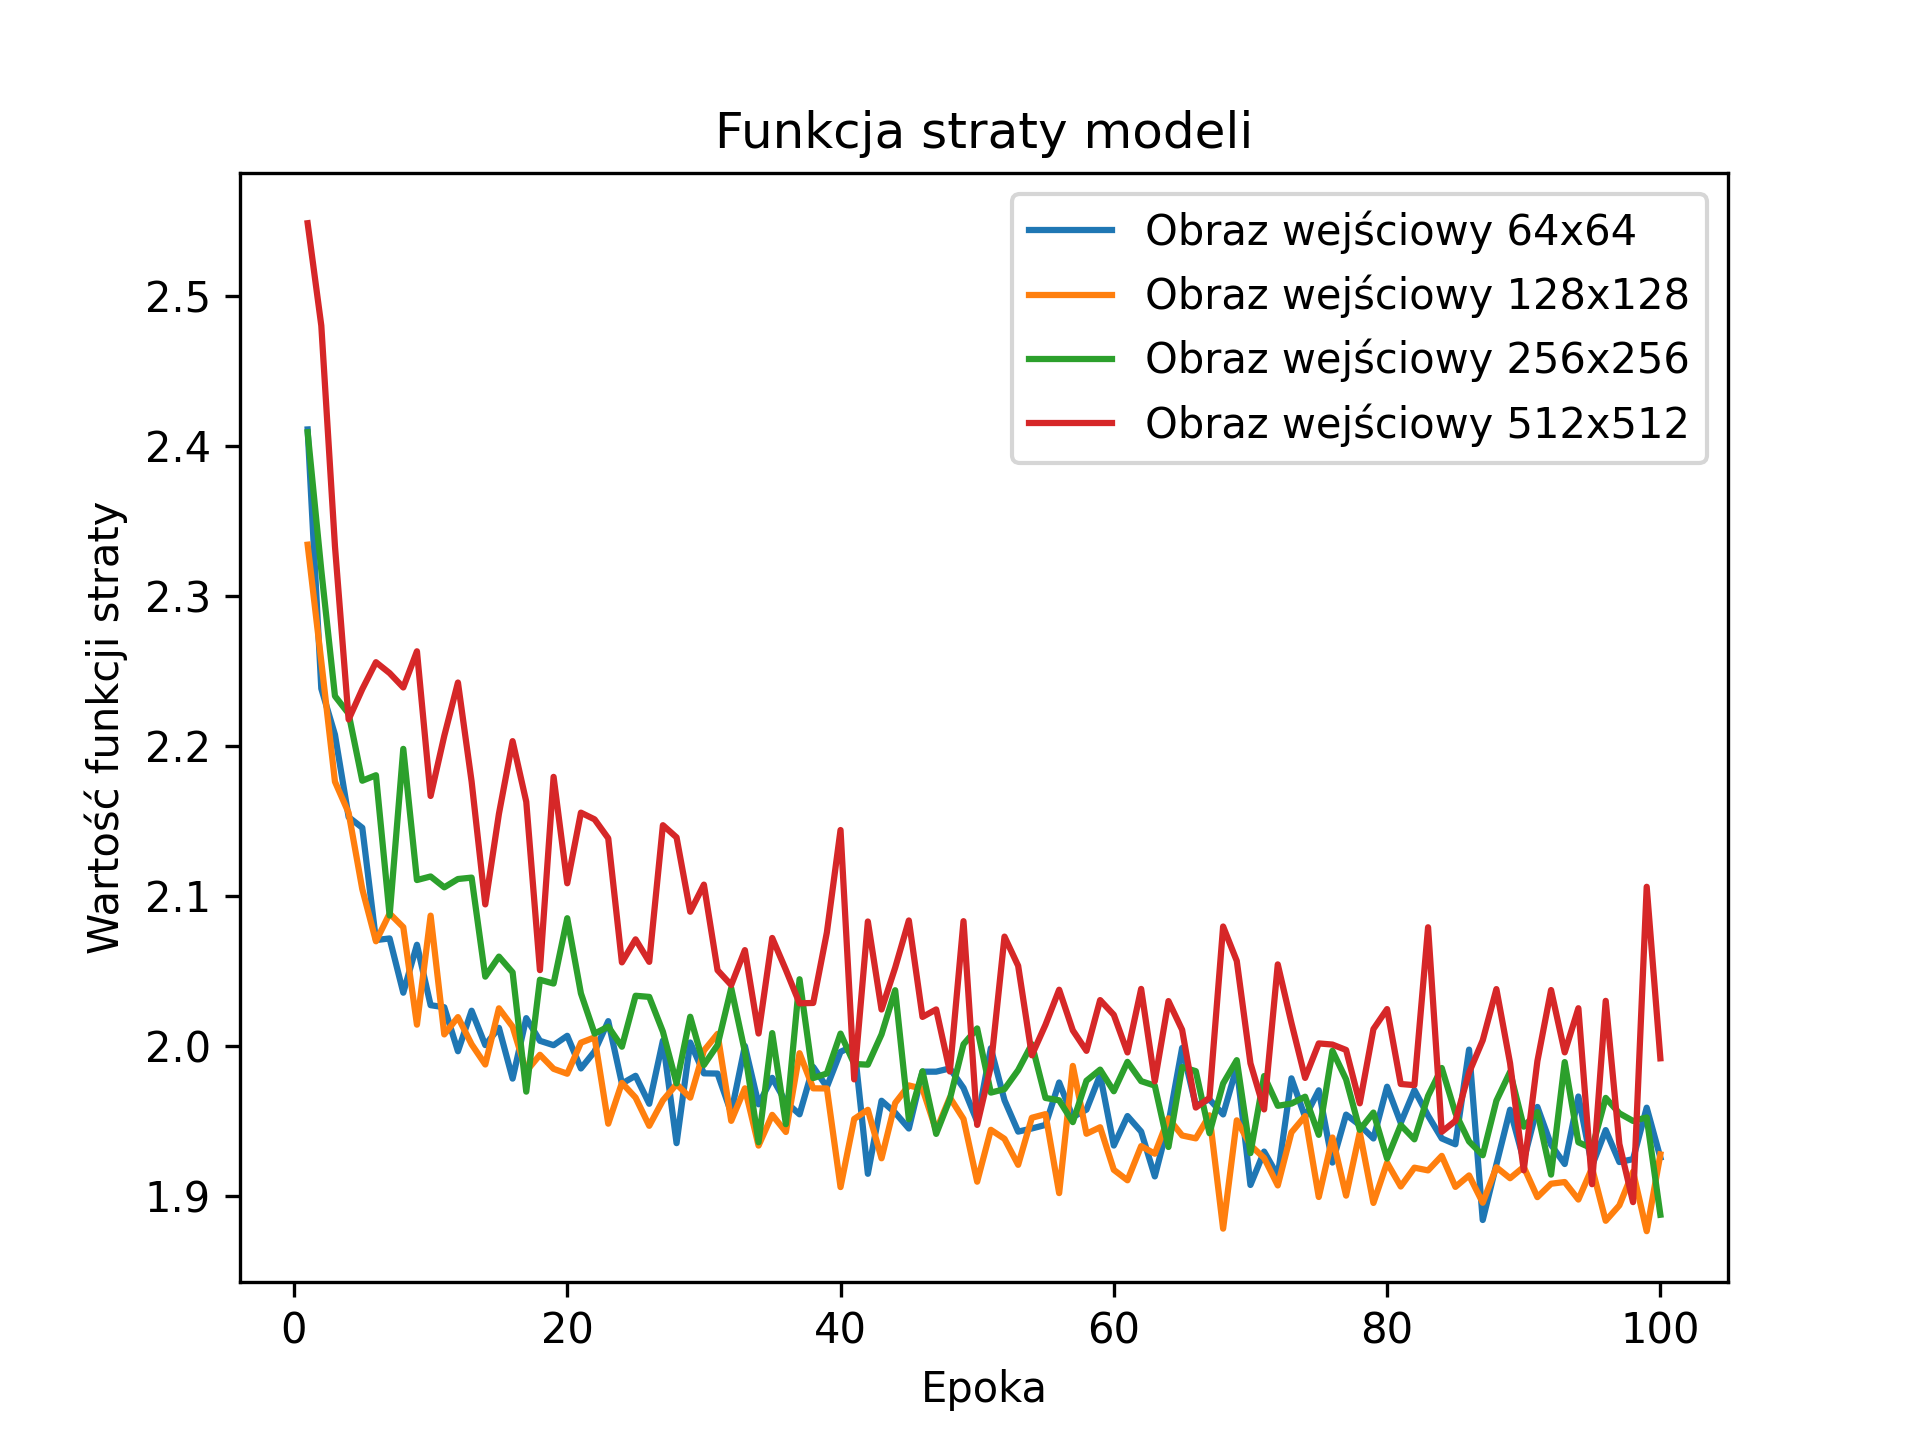
\includegraphics[width=0.7\columnwidth]{size.png}
	\caption{Funcja straty przy różnych rozmiarach segmentu wejściowego}
	\label{fig:size}
\end{center}
\end{figure}
Zauważyć można podobne wyniki dla segmentów o rozmiarze 64x64 oraz 128x128 pikseli.
Dla segmentu o rozmiarach 128x128 pikseli, błąd był nieznacznie niższy dla końcowych epok.
Jest to jednak skutkiem przetrenowania, gdyż wartość funkcji straty w zbiorze walidacyjnym była stała.
W przypadku segmentów o rozmiarze 512x512 pikseli nastąpiło znaczące pogorszenie wyników.
Rozważyć można wybór dowolnego z rozmiarów 64x64, 128x128 oraz 256x256 pikseli.
Należy jednak pamiętać, że mniejszy rozmiar segmentu wejściowego, choć przyśpiesza szkolenie,
proporcjonalnie wpływa na czas rekonstrukcję obrazu.

\section{Wyniki działania modelu}
Przedstawione zostały wyniki działania optymalnej sieci o 4 warstwach,
rozmiarze segmentu 256x256 oraz 8 pikselach przesunięcia przy rekonstrukcji.
\subsection{Roślinność na tle kamiennej ściany}
\begin{figure}[h!]
\begin{center}
	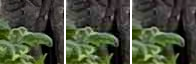
\includegraphics[width=0.85\columnwidth]{compare_sample.png}
	\caption{Segment oryginalny, skompresowany, oraz zrekonstruowany}
\end{center}
\end{figure}
\begin{figure}[h!]
\begin{center}
	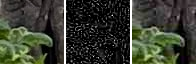
\includegraphics[width=0.85\columnwidth]{orig_vs_comp.png}
	\caption{Różnice między segmentem oryginalnym i skompresowanym}
\end{center}
\end{figure}
\begin{figure}[h!]
\begin{center}
	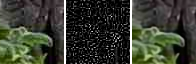
\includegraphics[width=0.85\columnwidth]{comp_vs_rest.png}
	\caption{Różnice między segmentem skompresowanym i zrekonstruowanym}
\end{center}
\end{figure}
\begin{figure}[h!]
\begin{center}
	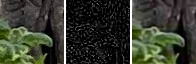
\includegraphics[width=0.85\columnwidth]{orig_vs_rest.png}
	\caption{Różnice między segmentem oryginalnym i zrekonstruowanym}
\end{center}
\end{figure}

\newpage
\subsection{Zarost na twarzy}
\begin{figure}[h!]
\begin{center}
	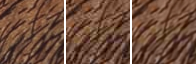
\includegraphics[width=0.85\columnwidth]{compare_sample2.png}
	\caption{Segment oryginalny, skompresowany, oraz zrekonstruowany}
\end{center}
\end{figure}
\begin{figure}[h!]
\begin{center}
	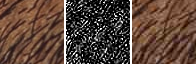
\includegraphics[width=0.85\columnwidth]{orig_vs_comp2.png}
	\caption{Różnice między segmentem oryginalnym i skompresowanym}
\end{center}
\end{figure}
\begin{figure}[h!]
\begin{center}
	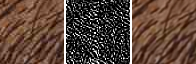
\includegraphics[width=0.85\columnwidth]{comp_vs_rest2.png}
	\caption{Różnice między segmentem skompresowanym i zrekonstruowanym}
\end{center}
\end{figure}
\begin{figure}[h!]
\begin{center}
	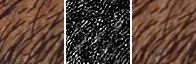
\includegraphics[width=0.85\columnwidth]{orig_vs_rest2.png}
	\caption{Różnice między segmentem oryginalnym i zrekonstruowanym}
\end{center}
\end{figure}
\subsection{Spostrzeżenia}
Zauważalna jest utrata detali względem segmentu oryginalnego, a nawet względem segmentu skompresowanego. Sieć ma cechy filtra uśredniającego.
W porównaniach widoczna jest siatka kwadratów o boku 8 pikseli, wynikająca ze sposobu działania algorytmu JPEG.
Różnica między segmentem oryginalnym i zrekonstruowanym jest mniejsza niż między segmentem oryginalnym i skompresowanym oraz skompresowanym i zrekonstruowanym.

\section{Rekonstrukcja pełnego obrazu}
Sieć została zaprojektowana do rekonstrukcji monochromatycznych segmentów o rozmiarze 256x256 pikseli.
Tworzy to potrzebę opracowania rozwiązania do przetwarzania obrazów o dowolnym rozmiarze.
Obraz zostaje podzielony na kanały RGB a następnie, kolejne segmenty każdej z warstw są rekonstruowane przez model.
Wartości otrzymanej macierzy są zaokrąglane do liczb całkowitych oraz następuje winsoryzacja wartości spoza zakresu 0-255.
W przypadku segmentów na krawędziach obrazu, brakujący fragment zostaje uzupełniony lustrzanym odbiciem obrazu a po rekonstrukcji odcięty.
Z podejściem wiąże się problem, widocznych granic między przetworzonymi segmentami.
Rozwiązaniem jest częściowe pokrycie segmentów przy przetwarzaniu oraz zastosowanie średniej ważonej na ich granicy Rys. \ref{fig:overlap}.
Wagi rzędów i kolumn rosną w głąb segmentu.
\\
\begin{figure}[h!]
\begin{center}
	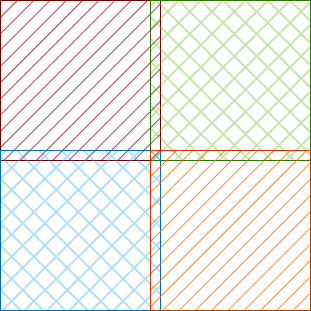
\includegraphics[width=0.4\columnwidth]{overlap.png}
	\caption{Nachodzace na siebie segmenty}
	\label{fig:overlap}
\end{center}
\end{figure}
\\
Pomimo zastosowania średniej ważonej, na granicy segmentów często pozostaje widoczna linnia.
Problem ten można rozwiązać poprzez wybranie odpowiedniej wartości przesunięcia segmentów.
Wpływ przesunięcia na obraz liczony był wartością średniego błędu bezwzględnego policzonego dla całego obrazu.
Zauważyć można spadek wartości dla przesunięcia o 8 i 16 pikseli Rys. \ref{fig:overlap_and_loss}.
Jest to związane z podziałem obrazu na obszary 8x8 przez algorytm JPEG.
Jeżeli krawędzie powstałe w wyniku rekonstrukcji obrazu pokryją się z krawędziami powstającymi przy kompresji,
wynikowy błąd będzie mniejszy niż w przypadku, gdyby na obrazie tworzyły się dodatkowe granice.
Dodatkowo widoczny jest spadek dla 11 pikseli, dla którego nie znam wyjaśnienia.
Wartość 8 pikseli została wybrana jako optymalna, przy większych wartościach pojawia się ryzyko rozmazania obrazu przez średnią ważoną.
\begin{figure}[h!]
\begin{center}
	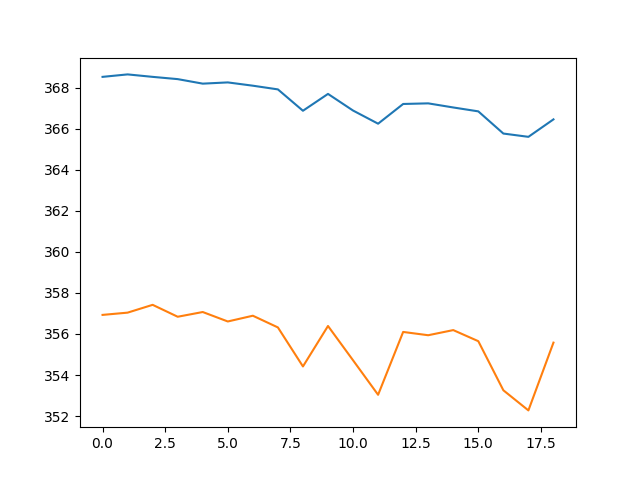
\includegraphics[width=0.7\columnwidth]{overlap_and_loss.png}
	\caption{Wartość funkcji błędu dla różnych wartości przesunięcia}
	\label{fig:overlap_and_loss}
\end{center}
\end{figure}
\section{Wnioski}
Można zastosować sieci typu U-Net do usuwania artefaktów kompresji stratnej.
Takie rozwiązanie jest jednak bardzo wolne. Przetworzenie obrazu o wymiarach 3024x4032 pikseli zajmuje około 80 sekund z wykorzystaniem karty graficznej Radeon RX 5700 XT.
Optymalne wydaje się zastosowanie sieci o 4 poziomach, przy rozmiarze segmentu wejściowego 256x256 pikseli.
Przy rekonstrukcji obrazu należy zastosować przesunięcie 8 pikseli,
aby granice między segmentami pokryły się z granicami powstałymi w wyniku działania algorytmu JPEG.
\bibliographystyle{plain}
\newpage
\bibliography{sprawozdanie}

\end{document}
